\section{}
The system shown in the figure is used to accurately measure changes when the pressure 
is increased by $\Delta P$ in the water pipe. When $\Delta h = 70$ mm, what is the change 
in the pipe pressure?

\begin{figure}[h]
    \centering
    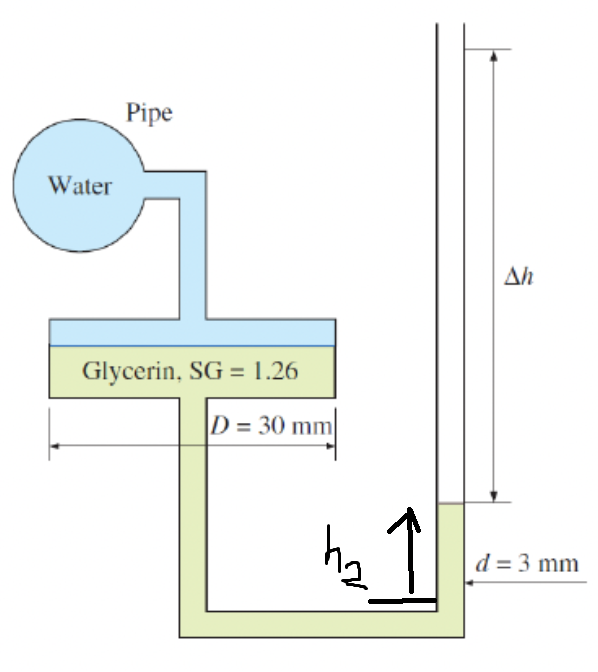
\includegraphics[width=0.3\textwidth]{Questions/Figures/Q3ProblemDiagram.png}
    \caption{Convoluted manometer diagram}
    \label{fig:Q3ProblemDiagram}
\end{figure}

For some pressure of water $P_{w}$ and a datum to measure the height of the glycerin $h_2$,
the pressure balance is given by:
\begin{align}
    P_{w, 1} - P_{atm} &= \rho_g g h_2 \label{eq:Q3State1} \\
    P_{w, 2} - P_{atm} &= \rho_g g (h_2 + \Delta h) \label{eq:Q3State2}
\end{align}

Observe that the width of the manometer does \textbf{not} contribute to the pressure balance.

Subtracting (\ref{eq:Q3State1}) from (\ref{eq:Q3State2}) yields:
\begin{equation}
    \Delta P = \rho_g g \Delta h \label{eq:Q3DeltaP}
\end{equation}

To find the density of glycerin given SG = 1.26, we can use the following equation:
\begin{equation}
    \rho_g = \rho_{H_2O} \times SG = 1000 \times 1.26 = \qty{1260}{\kilogram\per\meter\cubed}
\end{equation}

Substituting this into (\ref{eq:Q3DeltaP}) yields:
\begin{equation}
    \Delta P = 1260 \times 
    9.81 \times 0.07 
    = \boxed{\qty{865.2}{\pascal}} \nonumber
\end{equation}